\section{\langname{} engine}
This section deals with the basic designs of the engine, specifically its class framework and architecture, using a typical object-oriented design approach. First, the engine's overall architecture will be described, denoting the various layers in the structure with a brief explanation of their intent. Afterwards, two specific parts of the architecture will be described in greater detail. First, the \ac{api} as the interface outwards to compiler and frontend, and any desirable features it should have. Secondly, the engine that brings a start configuration to its conclusion - the overall control flow is described.

The language's syntax only describes half of the equation, and its semantics only describe how a battle should progress. With nothing but a compiler it would only be possible to parse and validate code before passing it to some arbitrary output language. Some run-time environment must be defined that is capable of making use of the output in some useful way. This could be done with an interpreter, a virtual machine or a run-time library. Either one would in principle enable the execution of code. We have chosen to work with the latter. A virtual machine would require a completely virtual processor to be designed and implemented, and an assembly language supported by the machine.
A run-time library allows for compile-time linkage with a separately designed backend, in effect "plugging" the \langname{} compiler output into an existing engine that will then proceed to resolve the battle scenario.

\subsection*{Architecture}

\begin{figure}
\centering
	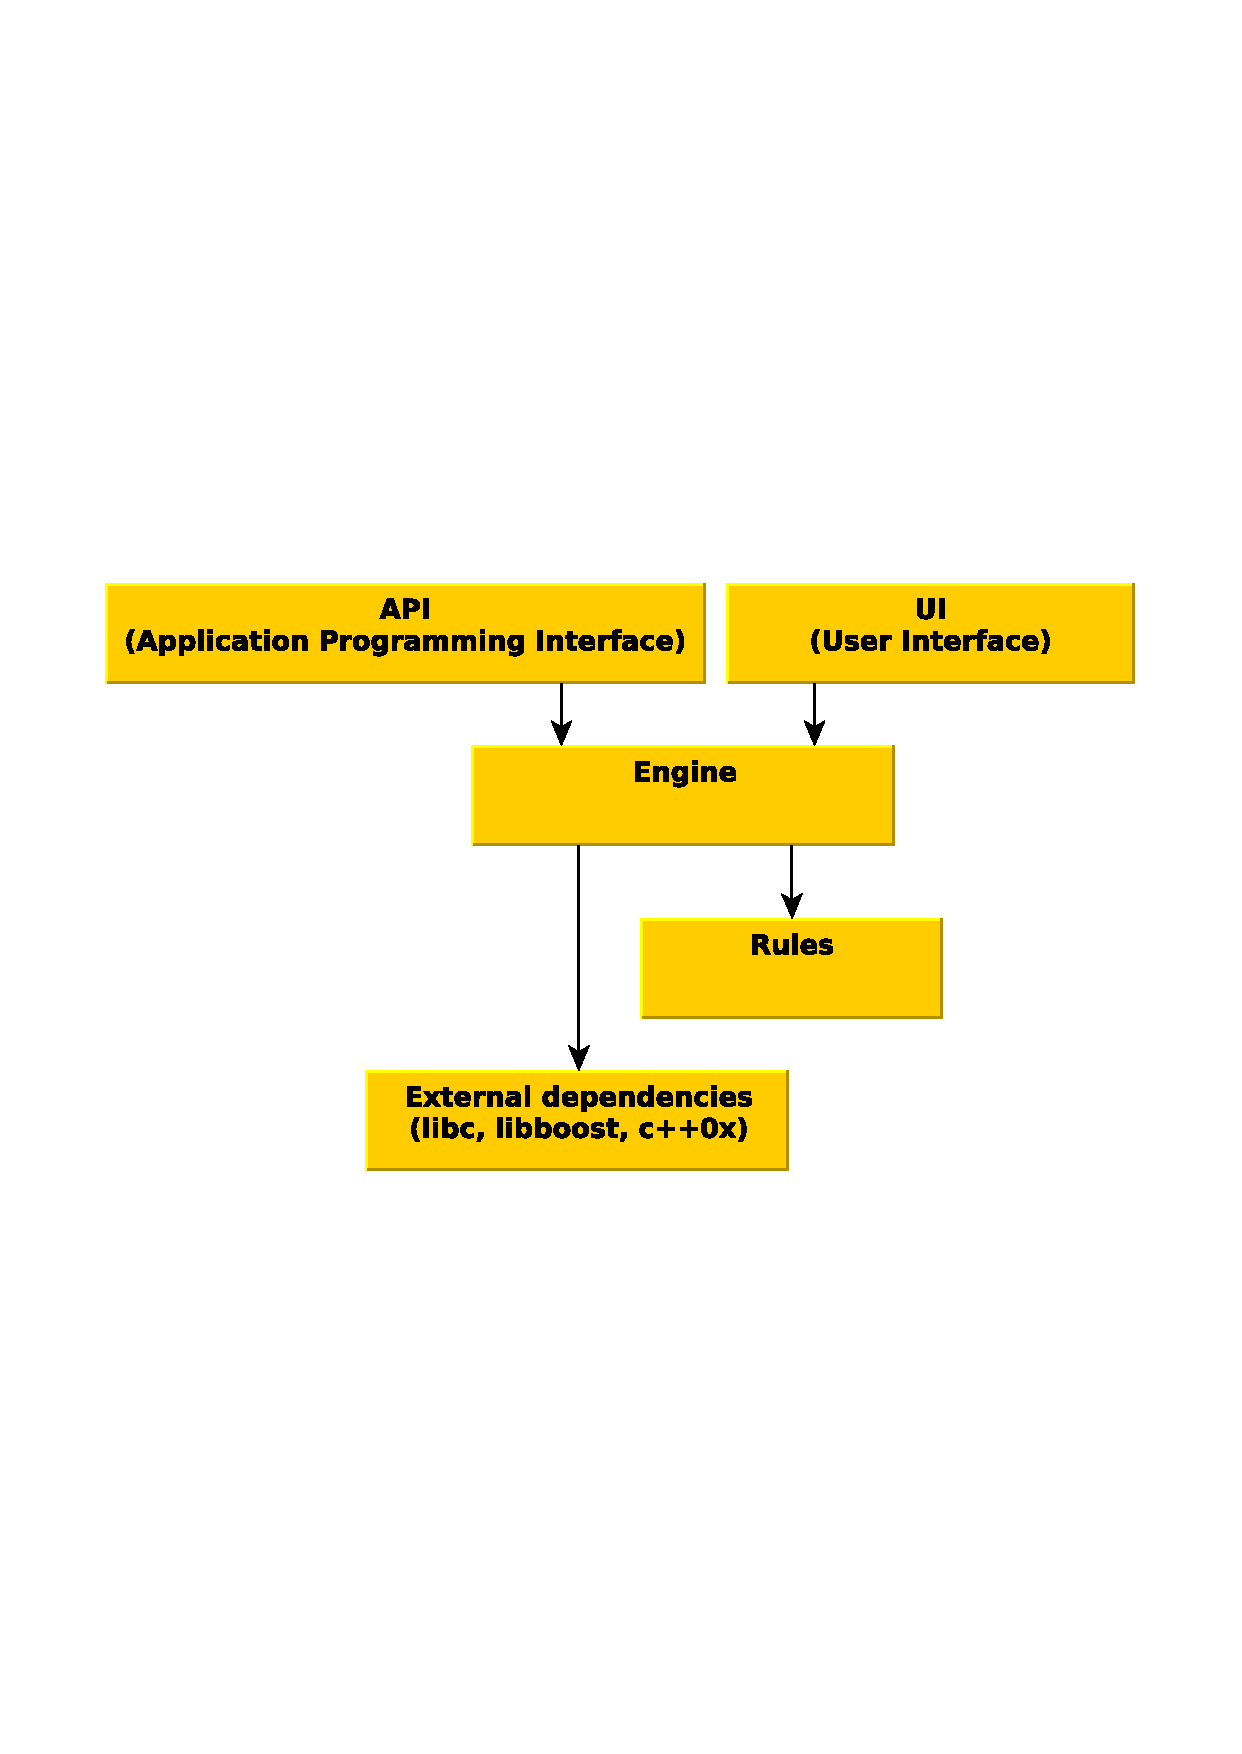
\includegraphics[scale=.4, clip=true, trim=2cm 10cm 2cm 10cm]{img/engine_architecture}
	\caption{\label{figure:design:engine:arch}The engine architecture.}
\end{figure}

To best consider the outwards visible classes, the intention of the engine should first be weighed in, along with a suggestion for its architecture.

The essential consideration is that the engine should support a clean and simple \ac{api} that the compiler can use in its templates for code generation. In particular, this is C++ representations of the base data types in \langname{}. Furthermore, the engine should implement the parts of \langname{} that have been pre-defined regardless of the individual program. This is the notion of turn-based actions and simple value-based intelligent agents \todo{What did we write in the theory/analysis about AI?}. Finally, some form of output must also be present, so the end-user and programmer can view the result of a scenario, if not also the intermediate turns. This can further be aided in implementation by creating a managed environment for all active \langname{} entities.

These considerations lead to an architecture as shown in Fig. \vref{figure:design:engine:arch}. A brief explanation of the components follows:

\begin{description}
	\item[The \ac{api}] is the parts of the engine that are exposed to other applications, and it is through this component that the compiler should describe the battle scenario. The \ac{api} encompasses a number of function and class declarations as well as several enumerators that map the data types and abstractions of \langname{} to the C++ engine.
	\item[The \ac{ui}] is the primary point of interaction for end-users of the engine. In this first iteration it is simply a stream that outputs and logs the actions of the engine based on the input battle scenario. A fuller design would extend the \ac{api} to sandwich it between \ac{ui} and a binary interface to allow game engines to control and read the engine state as a battle progresses (for a graphic game, this would be key).
	\item[Engine] The engine is intended to be the black box of scenario execution, accepting a series of scenario actors (Characters) and their definitions. It then proceeds to execute turns while streaming status and changes to the \ac{ui}.
	\item[Rules] were originally envisioned as external shared libraries to be plugged into the engine, either at link-time or compile-time, for game system features that were difficult or impossible to describe in \langname{} itself. Due to time constraints, we have opted for simplicity over flexibility and melded engine and rules into one. 
	\item[External dependencies] encompasses the libraries that the engine depends upon to be built and executed. It is mentioned in the architecture to clearly define where the \langname{} engine connects with the host system.
\end{description}

Of the five, the engine, rules and \ac{api} bear deeper explanation, as they represent core points of interest in regards to the project. The external dependencies are merely a formality, while the user interface is merely one of many options to observe the engine's state as it runs - another would be active debugging.

Note that while the designs presented in this section adequately describe the components in abstract form, several extensions must be applied before an effective implementation can be performed on a specific platform. This is deferred to the implementation chapter.

\subsection*{API}

The \ac{api} should expose parts of the engine that are relevant to the accurate definition of a battle scenario, and do so in an efficient, minimalist and easy-to-use manner. Perhaps the most obvious of approaches is to map the seven \langname{} primarchs to equivalent classes in the engine framework. This requires going through each of the classes, analyse their traits, and consider how they should be represented in a platform-independent manner, before finally being implemented in the compiler's target language - C++. Given the compositional nature of the primarchs, each class will be described in a bottom-up manner (smallest components first). The full class diagram can be seen on Fig. \vref{figure:language:engine:api_class}.

\begin{figure}
\centering
\includegraphics[scale=.6, clip=true, trim=1cm 4cm 1cm 4cm]{img/class_diagram_api}
\caption{\label{figure:language:engine:api_class}The \ac{api} class diagram, depicting abstractions of the seven basic compositional types of \langname{}.}
\end{figure}

\subsubsection*{Attribute}
The simplest of all primarchs, the Attribute basically represents a number value, and need not be more complex than such in the design phase.

\subsubsection*{Resource}
The Resource, like the Attribute, has a numbered \emph{current} value, but expands the definition with minimum and maximum values. One might consider the Resource as a specialised Attribute from this observation.

\subsubsection*{Behaviour}
Behaviours are simply sets of tuples combining a reference with a ratio, for example \textbf{owner.health} with the value $-3$. Similarly, this can be represented as a base class, Behaviour, that contains an unset number of BehaviourRatio objects, each with a \ac{rgr}/member reference and a numeric value.

\subsubsection*{Effect}
Effects are, like BehaviourRatio, tuples, combinations of targets and changes. An important factor that set the two apart is that Effect does not simply define a numbered change to the target, but instead a complete expression that may reference one or more other objects. For example, when calculating the physical damage done, a calculation involving the source Character's ''strength'' Attribute and ''weapon'' Item as well as their target's ''defense'' Attribute\todo{Check the calculation against the framework}.

\subsubsection*{Ability}
The Ability combines a set of Effects with a set of Costs and valid Targets. A Cost is a target/value tuple while a Target is an \ac{rgr}.

\subsubsection*{Event}
Events or, more correctly, event \emph{listeners} await the signalling of an event and reacts to it with a specific Ability, queued up for the next time the owning Character's turn is up.

\subsubsection*{Character}
The Character class assembles all the others into one whole definition, ready to be pitted against other Character objects. Thus, the Character should contain objects of all relevant primarchs. With the notable exception of the Behaviour primarch, a Character can contain zero or more of any primarch - the results of trying to combine several Behaviours into a single Character are undefined.

\subsubsection*{RGR}
The \ac{rgr} value types each bear different meanings according to scope and perspective, but have roughly the same function - they reference other objects. Thus it seems natural to have one base \ac{rgr} and let all possible \ac{rgr} types specialise from it. This is shown on \vref{figure:language:engine:rgr}

\begin{figure}
\centering
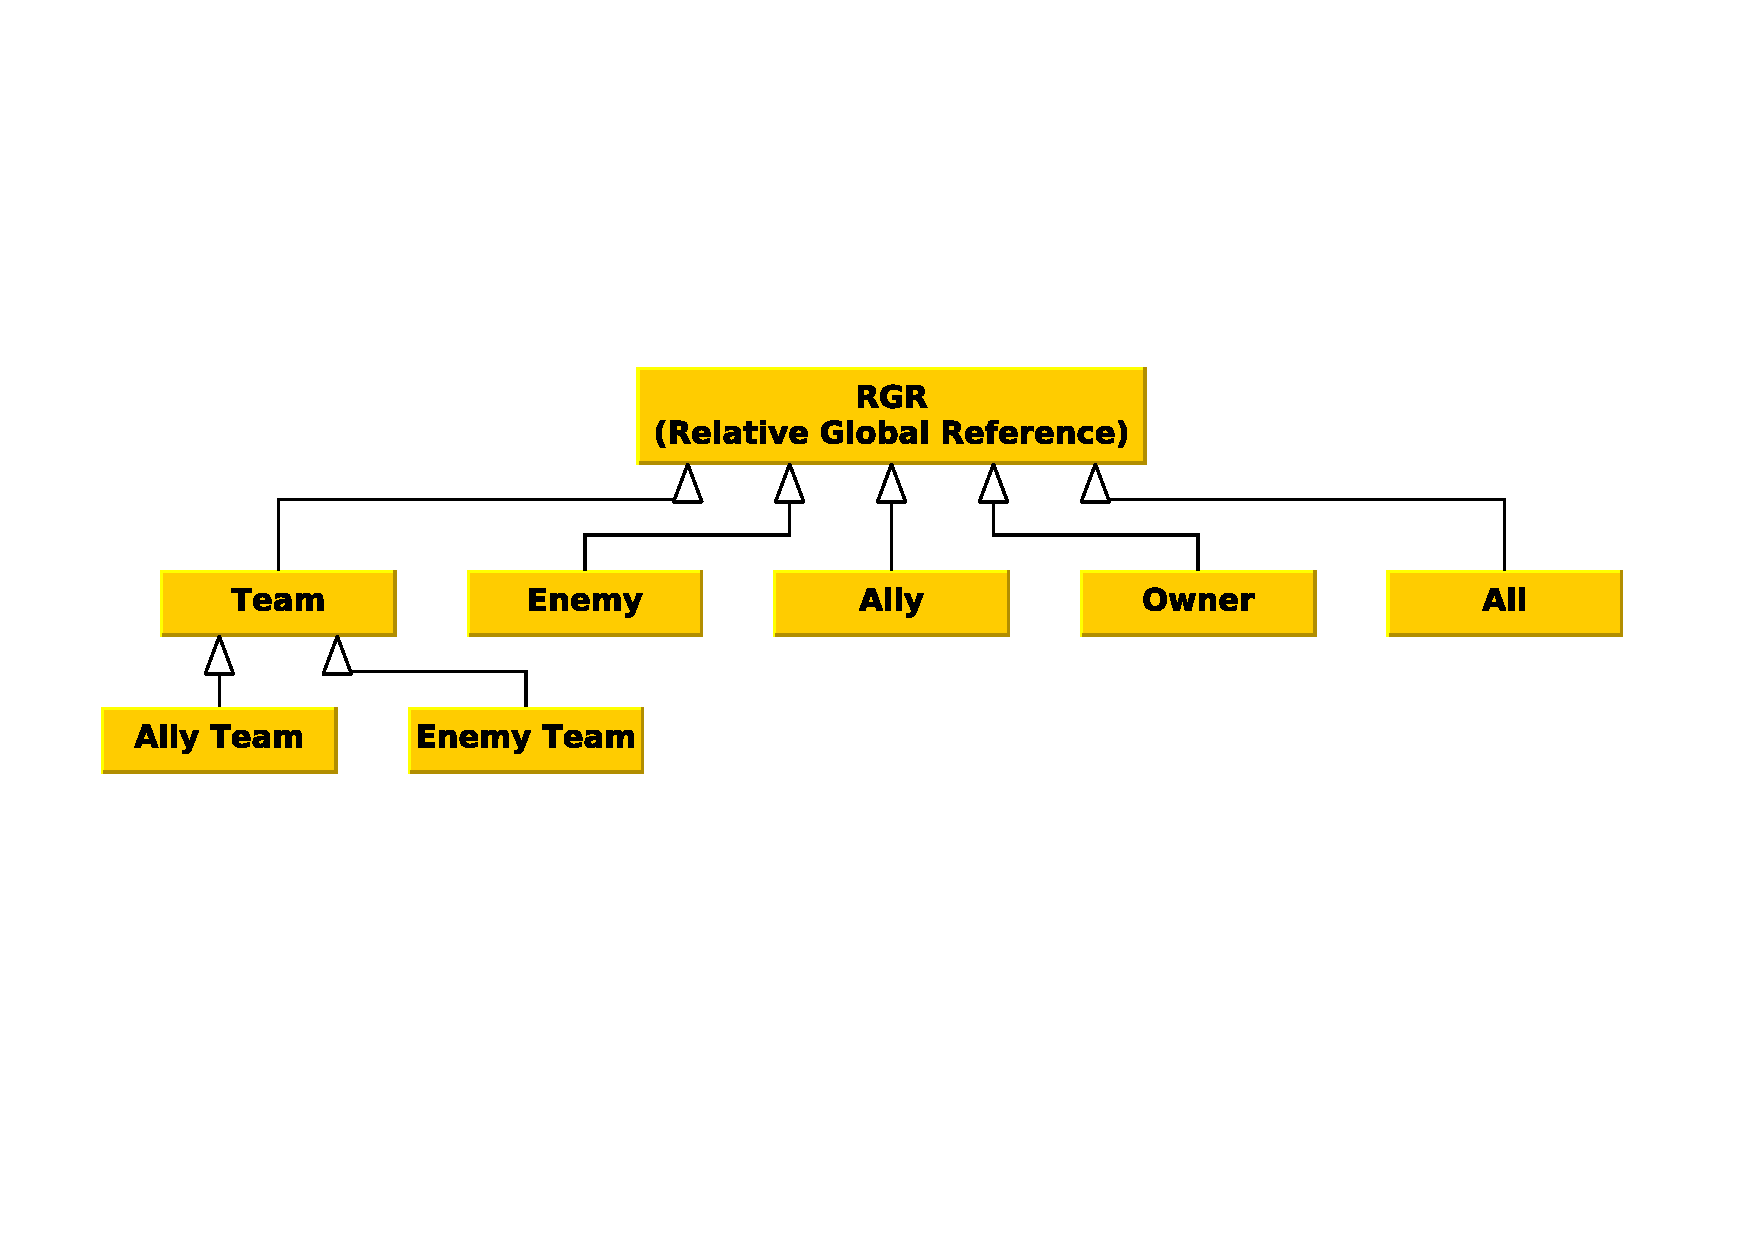
\includegraphics[scale=.4, clip=true, trim=0cm 8cm 0cm 6cm]{img/rgr_class_diagram}
\caption{\label{figure:language:engine:rgr}The \ac{rgr} class diagram.}
\end{figure}

\subsection{Engine}
With the primarchs now described as classes for the \ac{api}, it is possibly to more easily construct a similar design for the engine itself. The core features of the engine revolve around Character turns, decision-making based on Character Behaviours and \ac{rgr} support. The three are more intricately connected than the primarchs, and shown in brief on Fig. \vref{figure:design:engine:engine}

\begin{figure}
\centering
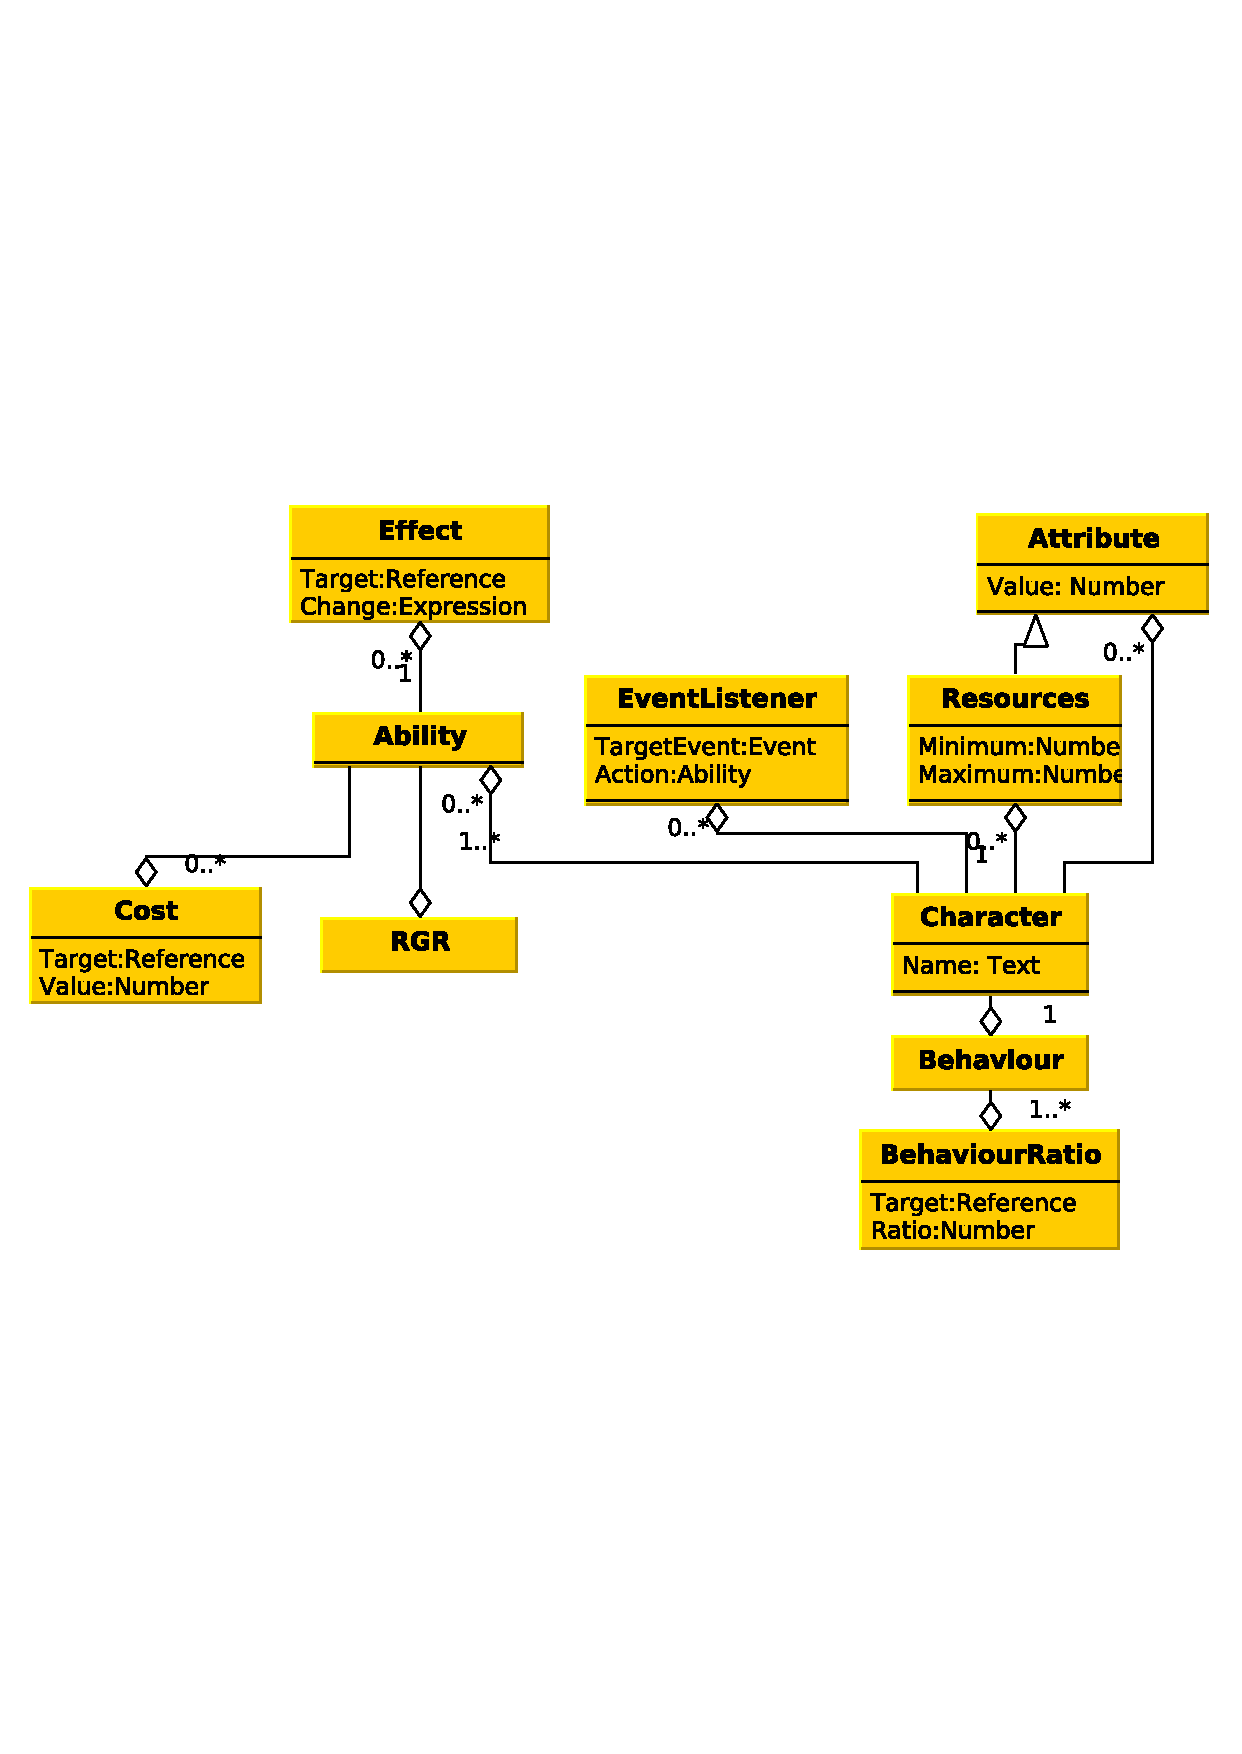
\includegraphics[scale=.5, clip=true, trim=0cm 8cm 1cm 8cm]{img/engine_class_diagram}
\caption{\label{figure:design:engine:engine}Class diagram for the engine itself}
\end{figure}

The engine will sequentially run turns for Characters that are still in play until the preset win condition is reached (as the semantics discuss, this can result in an infinite execution loop). Roughly, the engine's main workflow can be described thus:

\begin{enumerate}
	\item If the win condition is met, break and output end result.
	\item Get next Chararcter in turn order.
	\item For each valid Ability (one where the cost requirement is met):
	\begin{enumerate}
		\item Test each valid Ability target and record the resulting piggy value.
	\end{enumerate}
	\item The highest-scoring Ability/Target combination is realised in the scenario.
	\item Repeat.
\end{enumerate}

This loop is described in the flowchart on Fig. \vref{figure:design:engine:loop}

\begin{figure}[h]
\centering
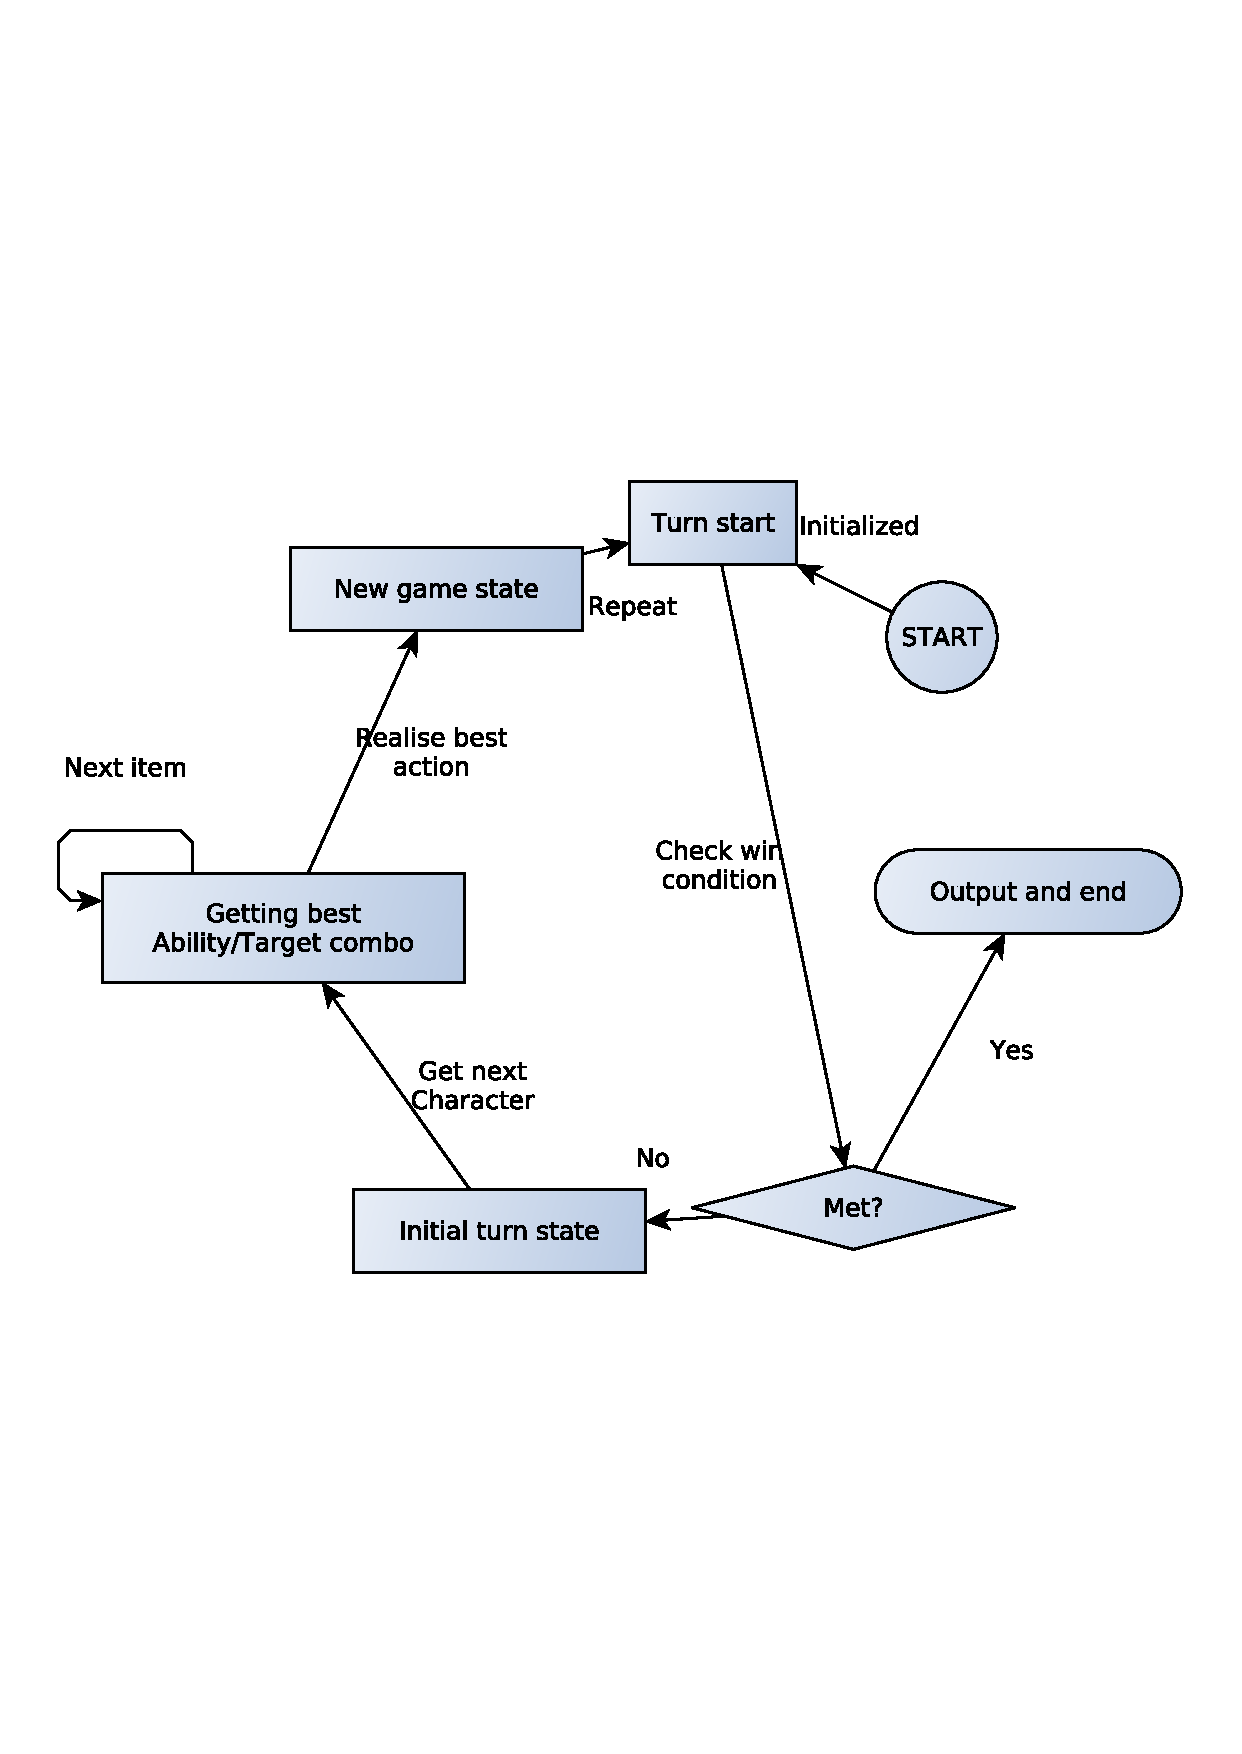
\includegraphics[scale=0.5, clip=true, trim=1cm 8cm 1cm 8cm]{img/engine_exec_loop}
\caption{\label{figure:design:engine:loop}The execution flow of the engine.}
\end{figure}

\subsection{Conclusion}
At this point the design of the engine architecture formally describes how the compiler and potential users should interact with and use the system. Furthermore, the stepped engine cycle